\subsection{Cấu trúc dự án}
\begin{itemize}
	\item \textbf{Frontend}:  
	Dự án frontend được tổ chức theo hướng module hóa, giúp dễ dàng mở rộng và tái sử dụng. Cấu trúc bao gồm:
    \begin{figure}[H]
        \centering
        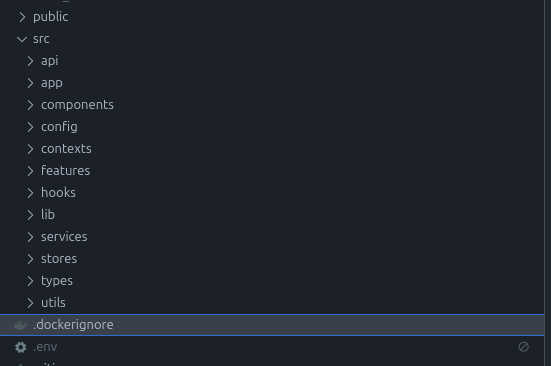
\includegraphics[width=15cm]{Images/hienthuc/cautrucfrontend.png}
        \vspace{0.5cm}
        \caption{Cấu trúc dự án frontend}
        \label{fig:frontend}
    \end{figure}
    \begin{itemize}
		\item \texttt{public/}: Lưu trữ tài nguyên tĩnh như ảnh, favicon, hoặc file tĩnh phục vụ trực tiếp cho ứng dụng.
		\item \texttt{src/}: Thư mục mã nguồn chính. Bên trong chia thành nhiều phần:
		\begin{itemize}
			\item \texttt{app/}: Định nghĩa các trang chính của ứng dụng, sử dụng App Router để điều hướng.
			\item \texttt{components/}: Chứa các component tái sử dụng chung trong toàn hệ thống.
			\item \texttt{contexts/}: Quản lý trạng thái toàn cục (ví dụ: trạng thái đăng nhập).
			\item \texttt{features/}: Mỗi tính năng được chia riêng, gồm:
			\begin{itemize}
				\item \texttt{components/}: Component riêng cho từng tính năng.
				\item \texttt{api/}: Gọi và quản lý API cho tính năng.
			\end{itemize}
			\item \texttt{hooks/}: Chứa các custom hooks hỗ trợ tái sử dụng logic React.
			\item \texttt{lib/}: Định nghĩa hàm tiện ích, xử lý logic chung.
			\item \texttt{services/}: Đảm nhận xử lý nghiệp vụ phía frontend và giao tiếp với backend.
		\end{itemize}
	\end{itemize}

	\item \textbf{Backend}:  
	Dự án backend sử dụng kiến trúc chia module và library, giúp đảm bảo tính rõ ràng, dễ quản lý và mở rộng. Cấu trúc bao gồm:
    \begin{figure}[H]
        \centering
        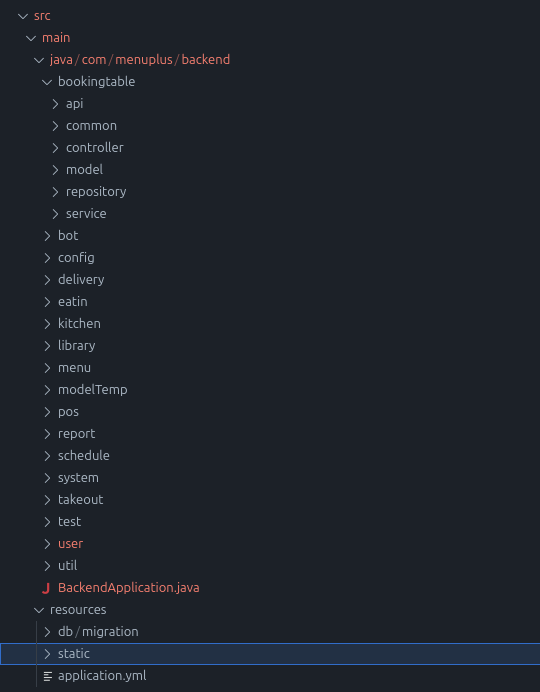
\includegraphics[width=15cm]{Images/hienthuc/cautrucbackend.png}
        \vspace{0.5cm}
        \caption{Cấu trúc dự án backend}
        \label{fig:backend}
    \end{figure}
	\begin{itemize}
		\item \texttt{src/main/java/.../backend/}: Mã nguồn chính, chia theo domain/tính năng (modules).
		\begin{itemize}
			\item \texttt{api/}: Chứa API service, DTO, mapper để giao tiếp với frontend.
			\item \texttt{common/}: Định nghĩa các thành phần dùng chung (ví dụ: API message).
			\item \texttt{model/}: Khai báo các lớp dữ liệu và entity.
			\item \texttt{repository/}: Quản lý truy xuất dữ liệu từ cơ sở dữ liệu.
			\item \texttt{service/}: Chứa logic nghiệp vụ của hệ thống.
		\end{itemize}
		\item Library toàn hệ thống:
		\begin{itemize}
			\item \texttt{util/}: Hàm tiện ích dùng chung.
			\item \texttt{exception/}: Xử lý lỗi, ngoại lệ hệ thống.
			\item \texttt{security/}: Cấu hình và xử lý liên quan đến bảo mật.
			\item \texttt{config/}: Cấu hình ứng dụng (Spring Boot, database, bảo mật,...).
		\end{itemize}
		\item \texttt{resources/}: Chứa cấu hình \texttt{application.yml}, migration scripts, và static resources.
	\end{itemize}
\end{itemize}

\subsection{Cách chạy dự án}
\begin{itemize}
	\item \textbf{Backend}:  
	Mã nguồn backend được quản lý tại \url{https://github.com/DATN-HH/back-end}.  
	\begin{enumerate}
		\item Clone repository:
		\begin{verbatim}
git clone https://github.com/DATN-HH/back-end.git
cd back-end
		\end{verbatim}

		\item Thiết lập các biến môi trường trong hệ thống hoặc trong \texttt{application.yml}:
		\begin{verbatim}
# Database
MP_DB_URL=jdbc:postgresql://localhost:5432/menuplus
MP_DB_USERNAME=postgres
MP_DB_PASSWORD=12345

# Redis
MP_REDIS_URL=redis://localhost:6379
MP_REDIS_PASSWORD=
MP_REDIS_DATABASE=0
MP_REDIS_TIMEOUT=600000

# JWT Authentication
MP_AUTH_JWT_SECRET=your_jwt_secret
MP_AUTH_JWT_EXPIRE=864000000

# Payment (PayOS)
MP_PAYMENT_CLIENT_ID=your_client_id
MP_PAYMENT_API_KEY=your_api_key
MP_PAYMENT_CHECKSUM_KEY=your_checksum_key
MP_PAYMENT_RETURN_URL=http://localhost:3000/payment/success
MP_PAYMENT_CANCEL_URL=http://localhost:3000/payment/cancel

# Cloudinary
MP_CLOUDINARY_CLOUD_NAME=your_cloud_name
MP_CLOUDINARY_API_KEY=your_api_key
MP_CLOUDINARY_API_SECRET=your_api_secret
MP_CLOUDINARY_SECURE=true
MP_CLOUDINARY_UPLOAD_FOLDER=menuplus
MP_CLOUDINARY_DEFAULT_QUALITY=auto
MP_CLOUDINARY_DEFAULT_FORMAT=jpg

# Email
EMAIL_SMTP_HOST=smtp.gmail.com
EMAIL_SMTP_PORT=587
EMAIL_SMTP_USERNAME=your_email@gmail.com
EMAIL_SMTP_PASSWORD=your_password
EMAIL_FROM_ADDRESS=your_email@gmail.com
EMAIL_FROM_NAME=MenuPlus System
		\end{verbatim}

		\item Chạy ứng dụng backend:
		\begin{verbatim}
mvn spring-boot:run
		\end{verbatim}
	\end{enumerate}

	\item \textbf{Frontend}:  
	Mã nguồn frontend được quản lý tại \url{https://github.com/DATN-HH/front-end}.  
	\begin{enumerate}
		\item Clone repository:
		\begin{verbatim}
git clone https://github.com/DATN-HH/front-end.git
cd front-end
		\end{verbatim}

		\item Tạo file \texttt{.env.local} và thêm các biến môi trường:
		\begin{verbatim}
NEXT_PUBLIC_API_URL=http://localhost:8090
NEXT_PUBLIC_API_FRONTEND=http://localhost:3000
		\end{verbatim}

		\item Cài đặt dependencies:
		\begin{verbatim}
npm install
		\end{verbatim}

		\item Khởi chạy ứng dụng frontend:
		\begin{verbatim}
npm run dev
		\end{verbatim}
	\end{enumerate}
\end{itemize}

\subsection{Một số luồng chính}\label{subsec:mot-so-luong-chinh}

\begin{figure}[H]
    \centering
    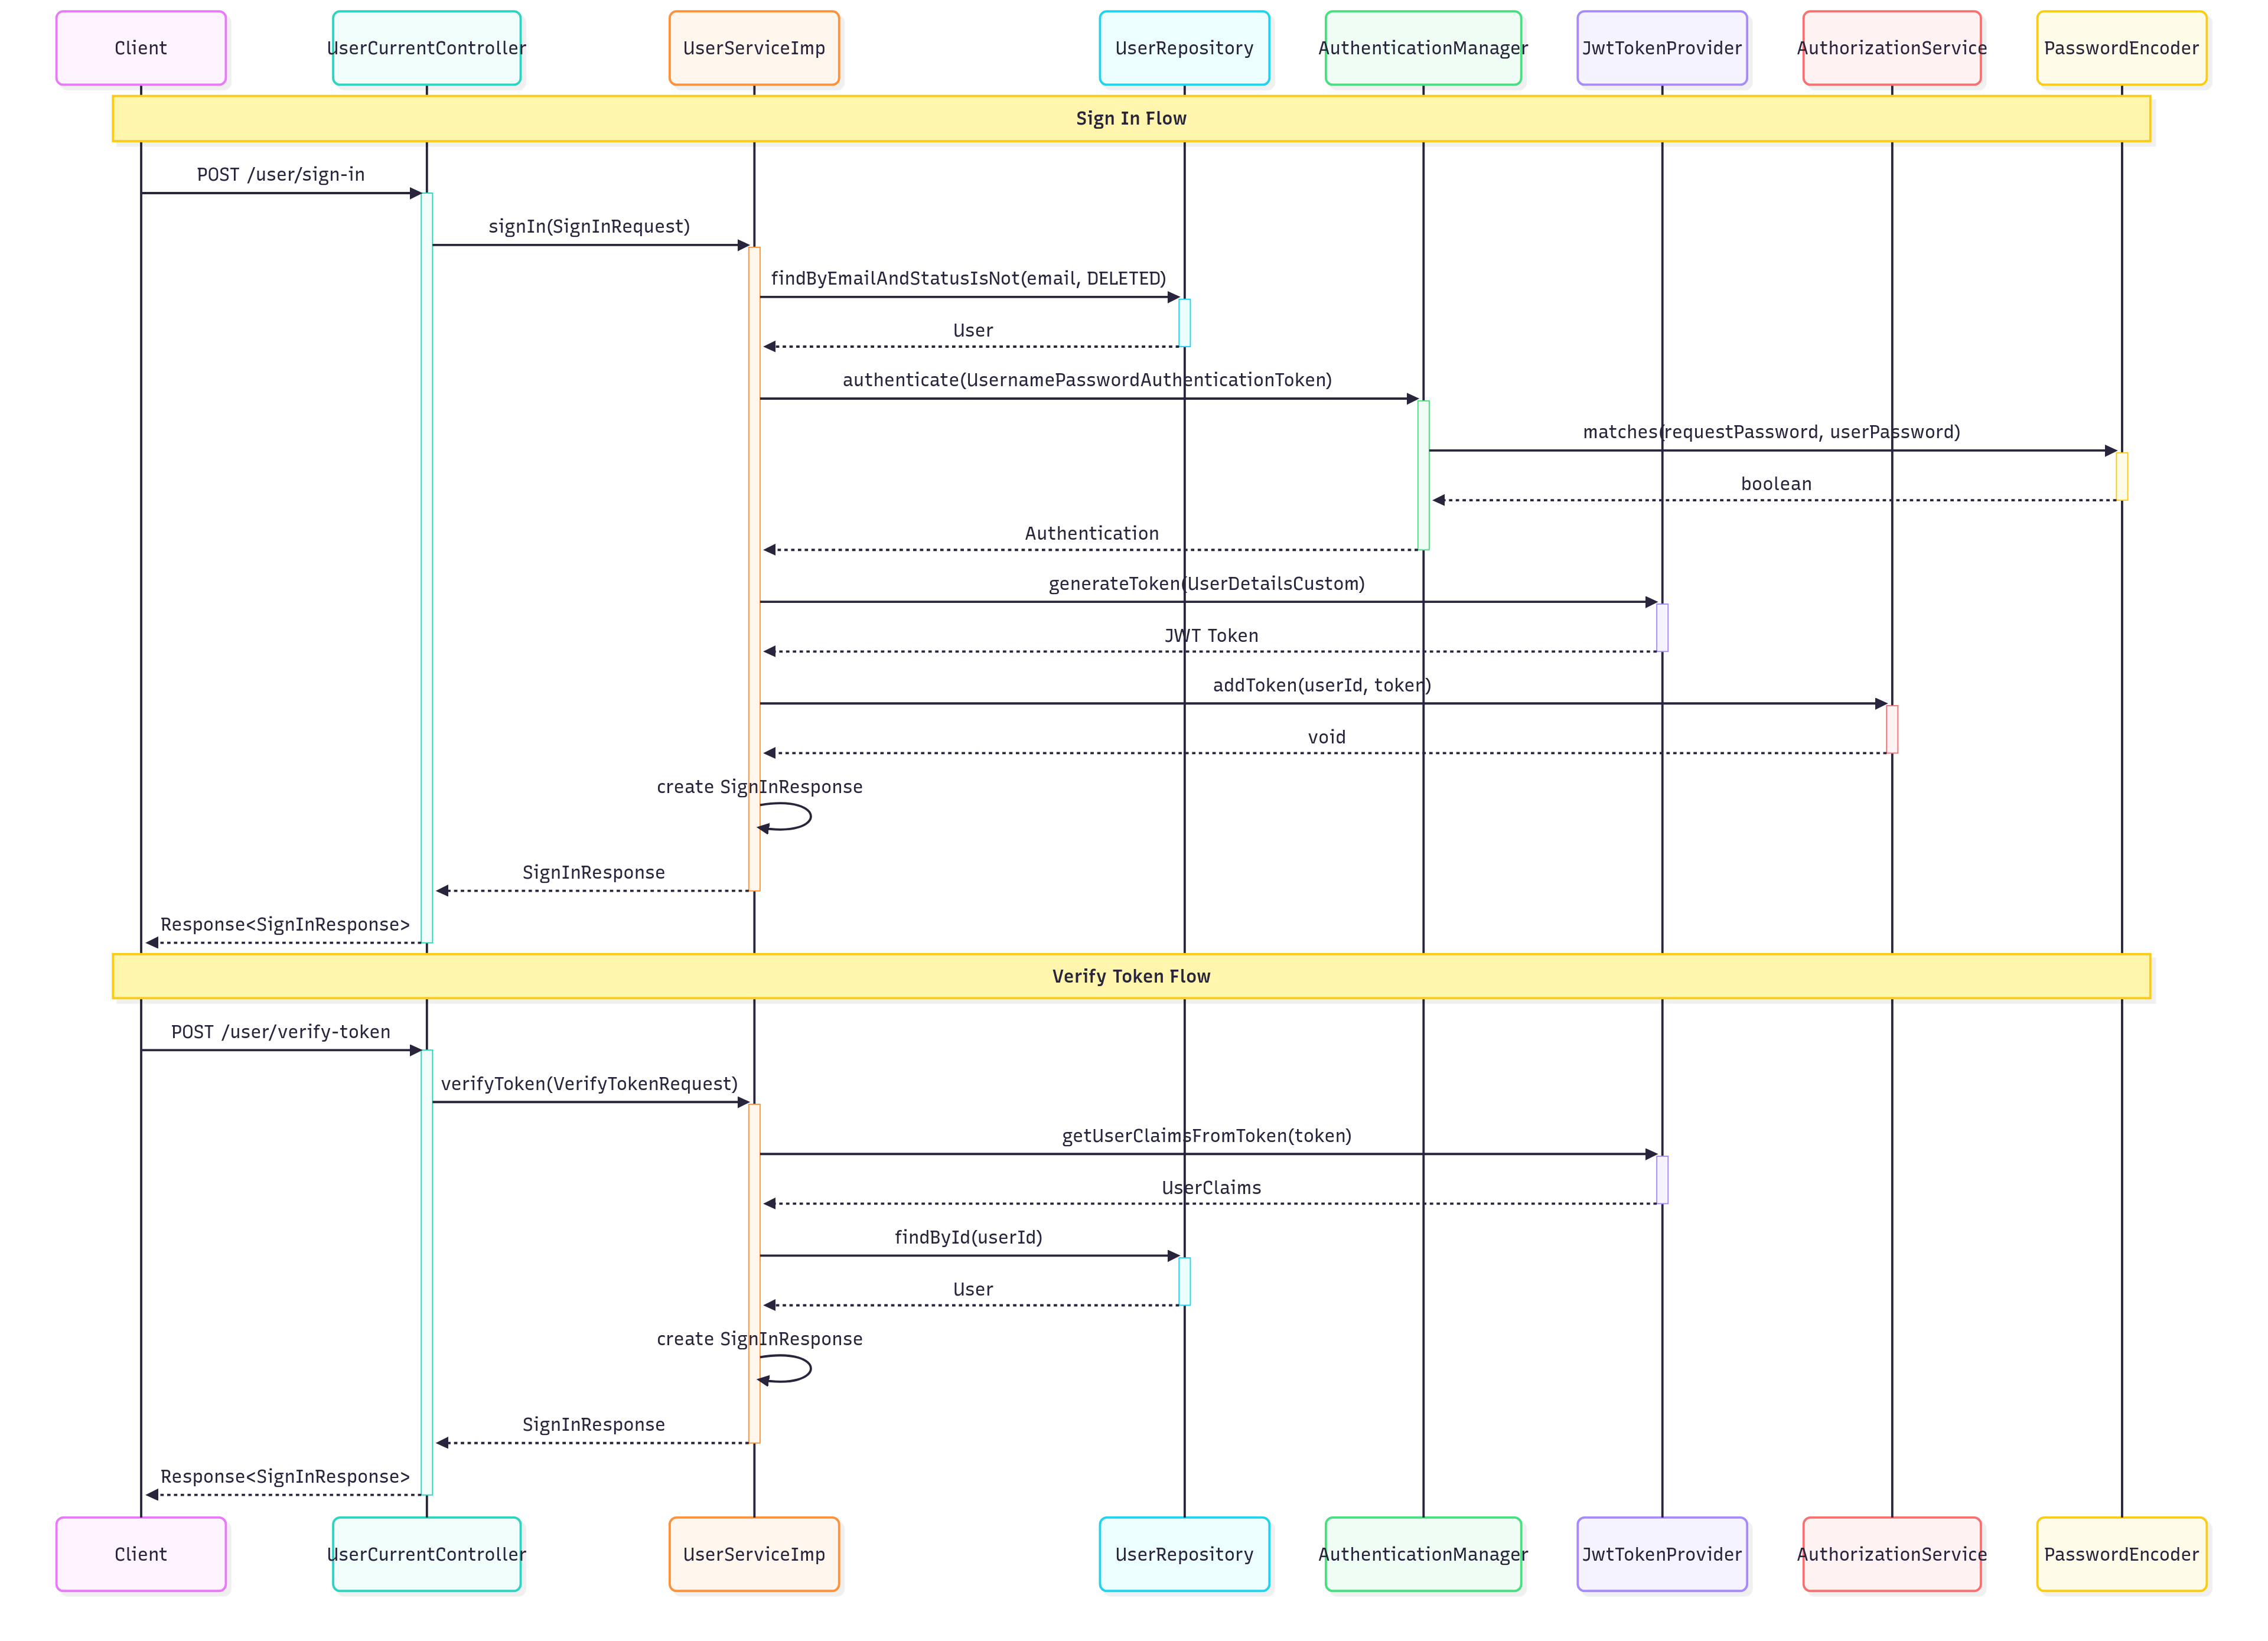
\includegraphics[width=\linewidth]{Images/diagram/Authen_sequence}
    \vspace{0.5cm}
    \caption{Sequence diagram: Xác thực người dùng}
    \label{fig:my_label}
\end{figure}
\begin{figure}[H]
    \centering
    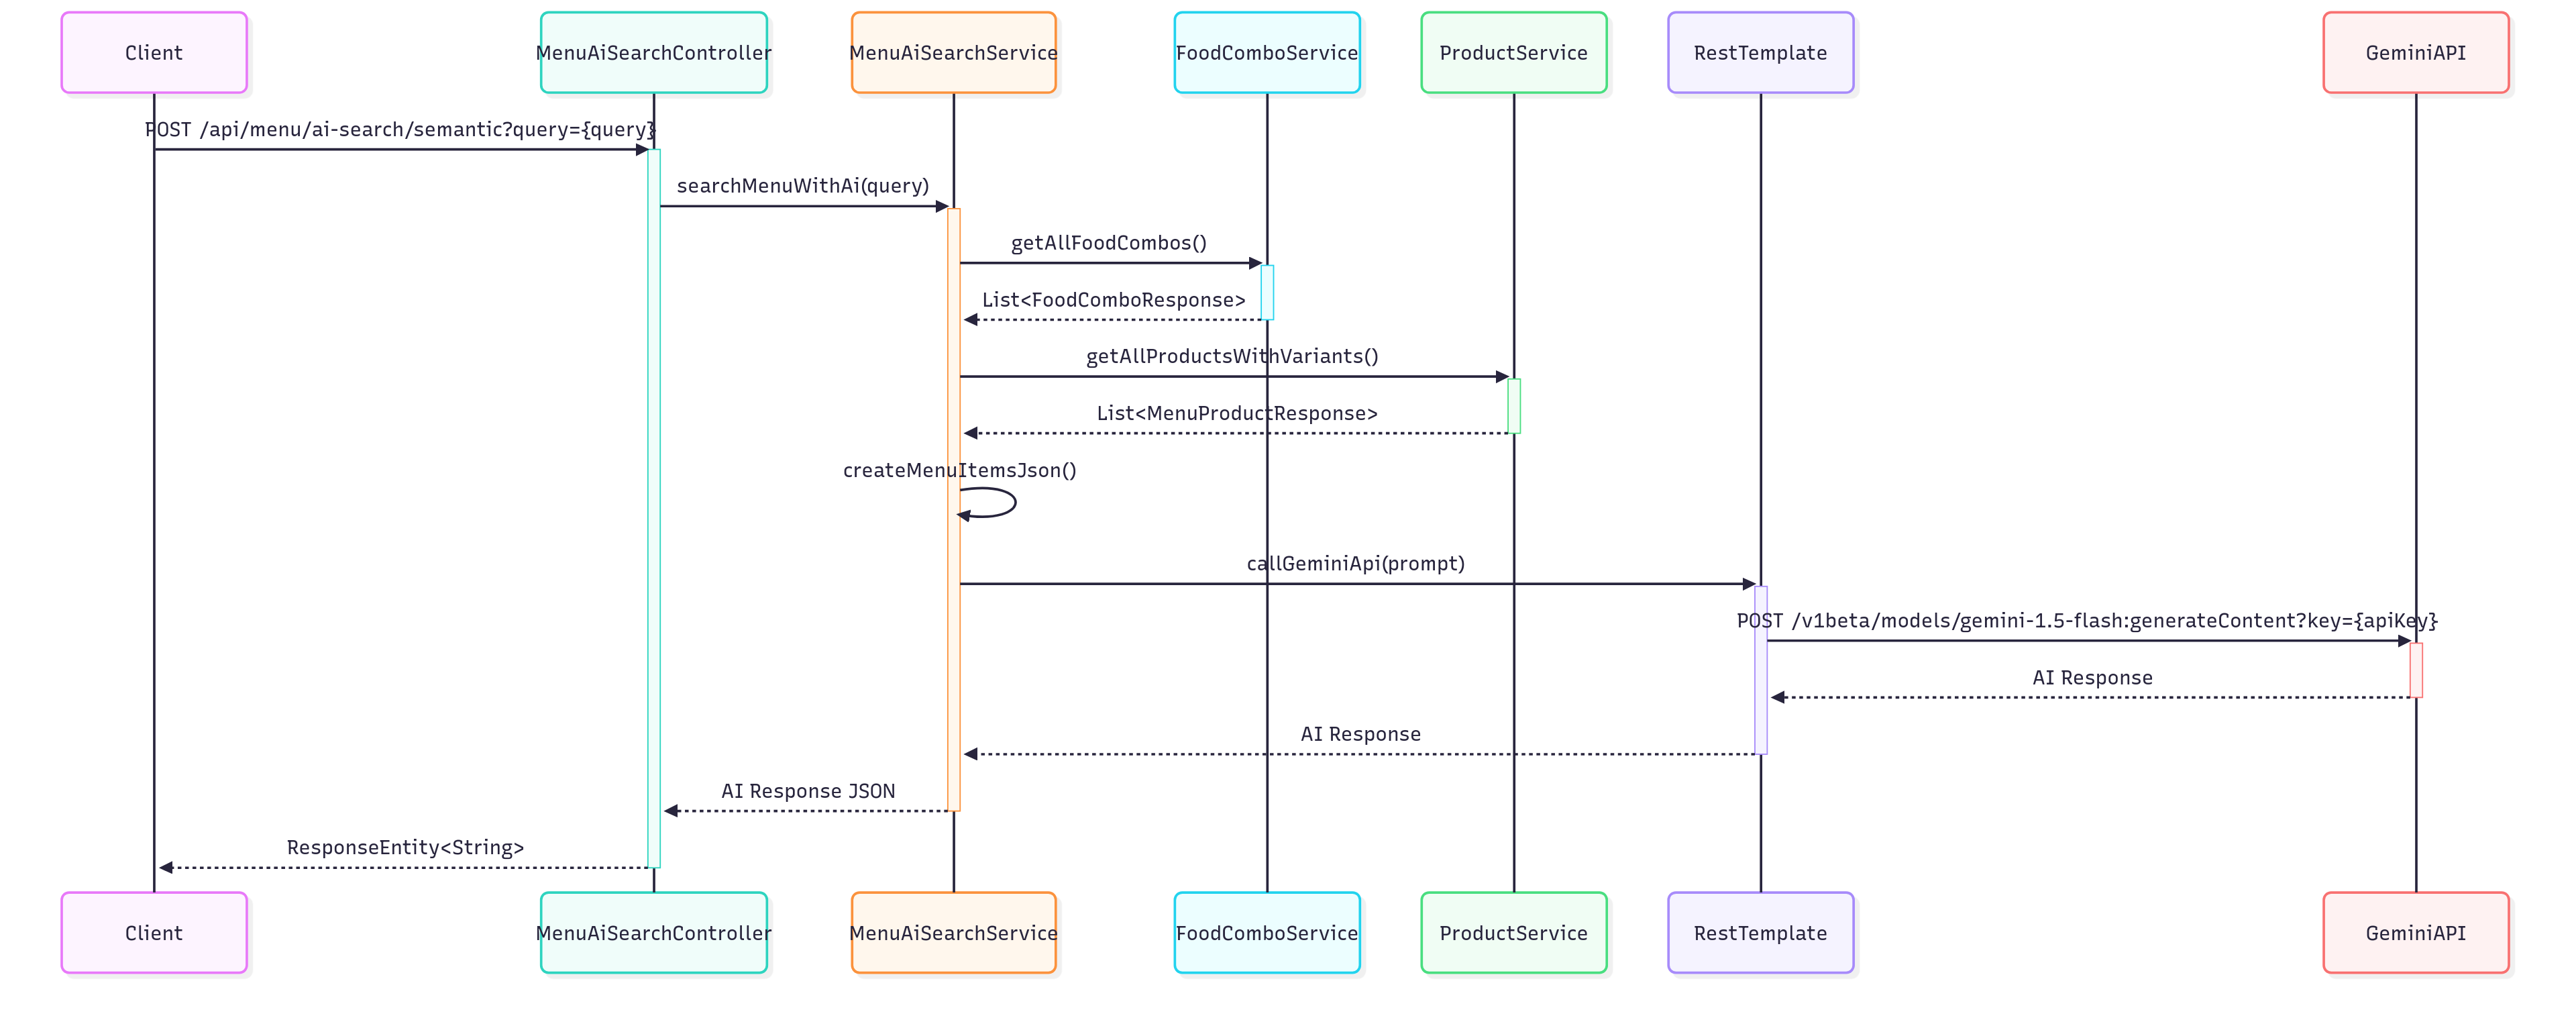
\includegraphics[width=\linewidth]{Images/diagram/AI_search_Seq}
    \vspace{0.5cm}
    \caption{Sequence diagram: Tìm kiếm thực đơn (AI)}
    \label{fig:my_label}
\end{figure}
\begin{figure}[H]
    \centering
    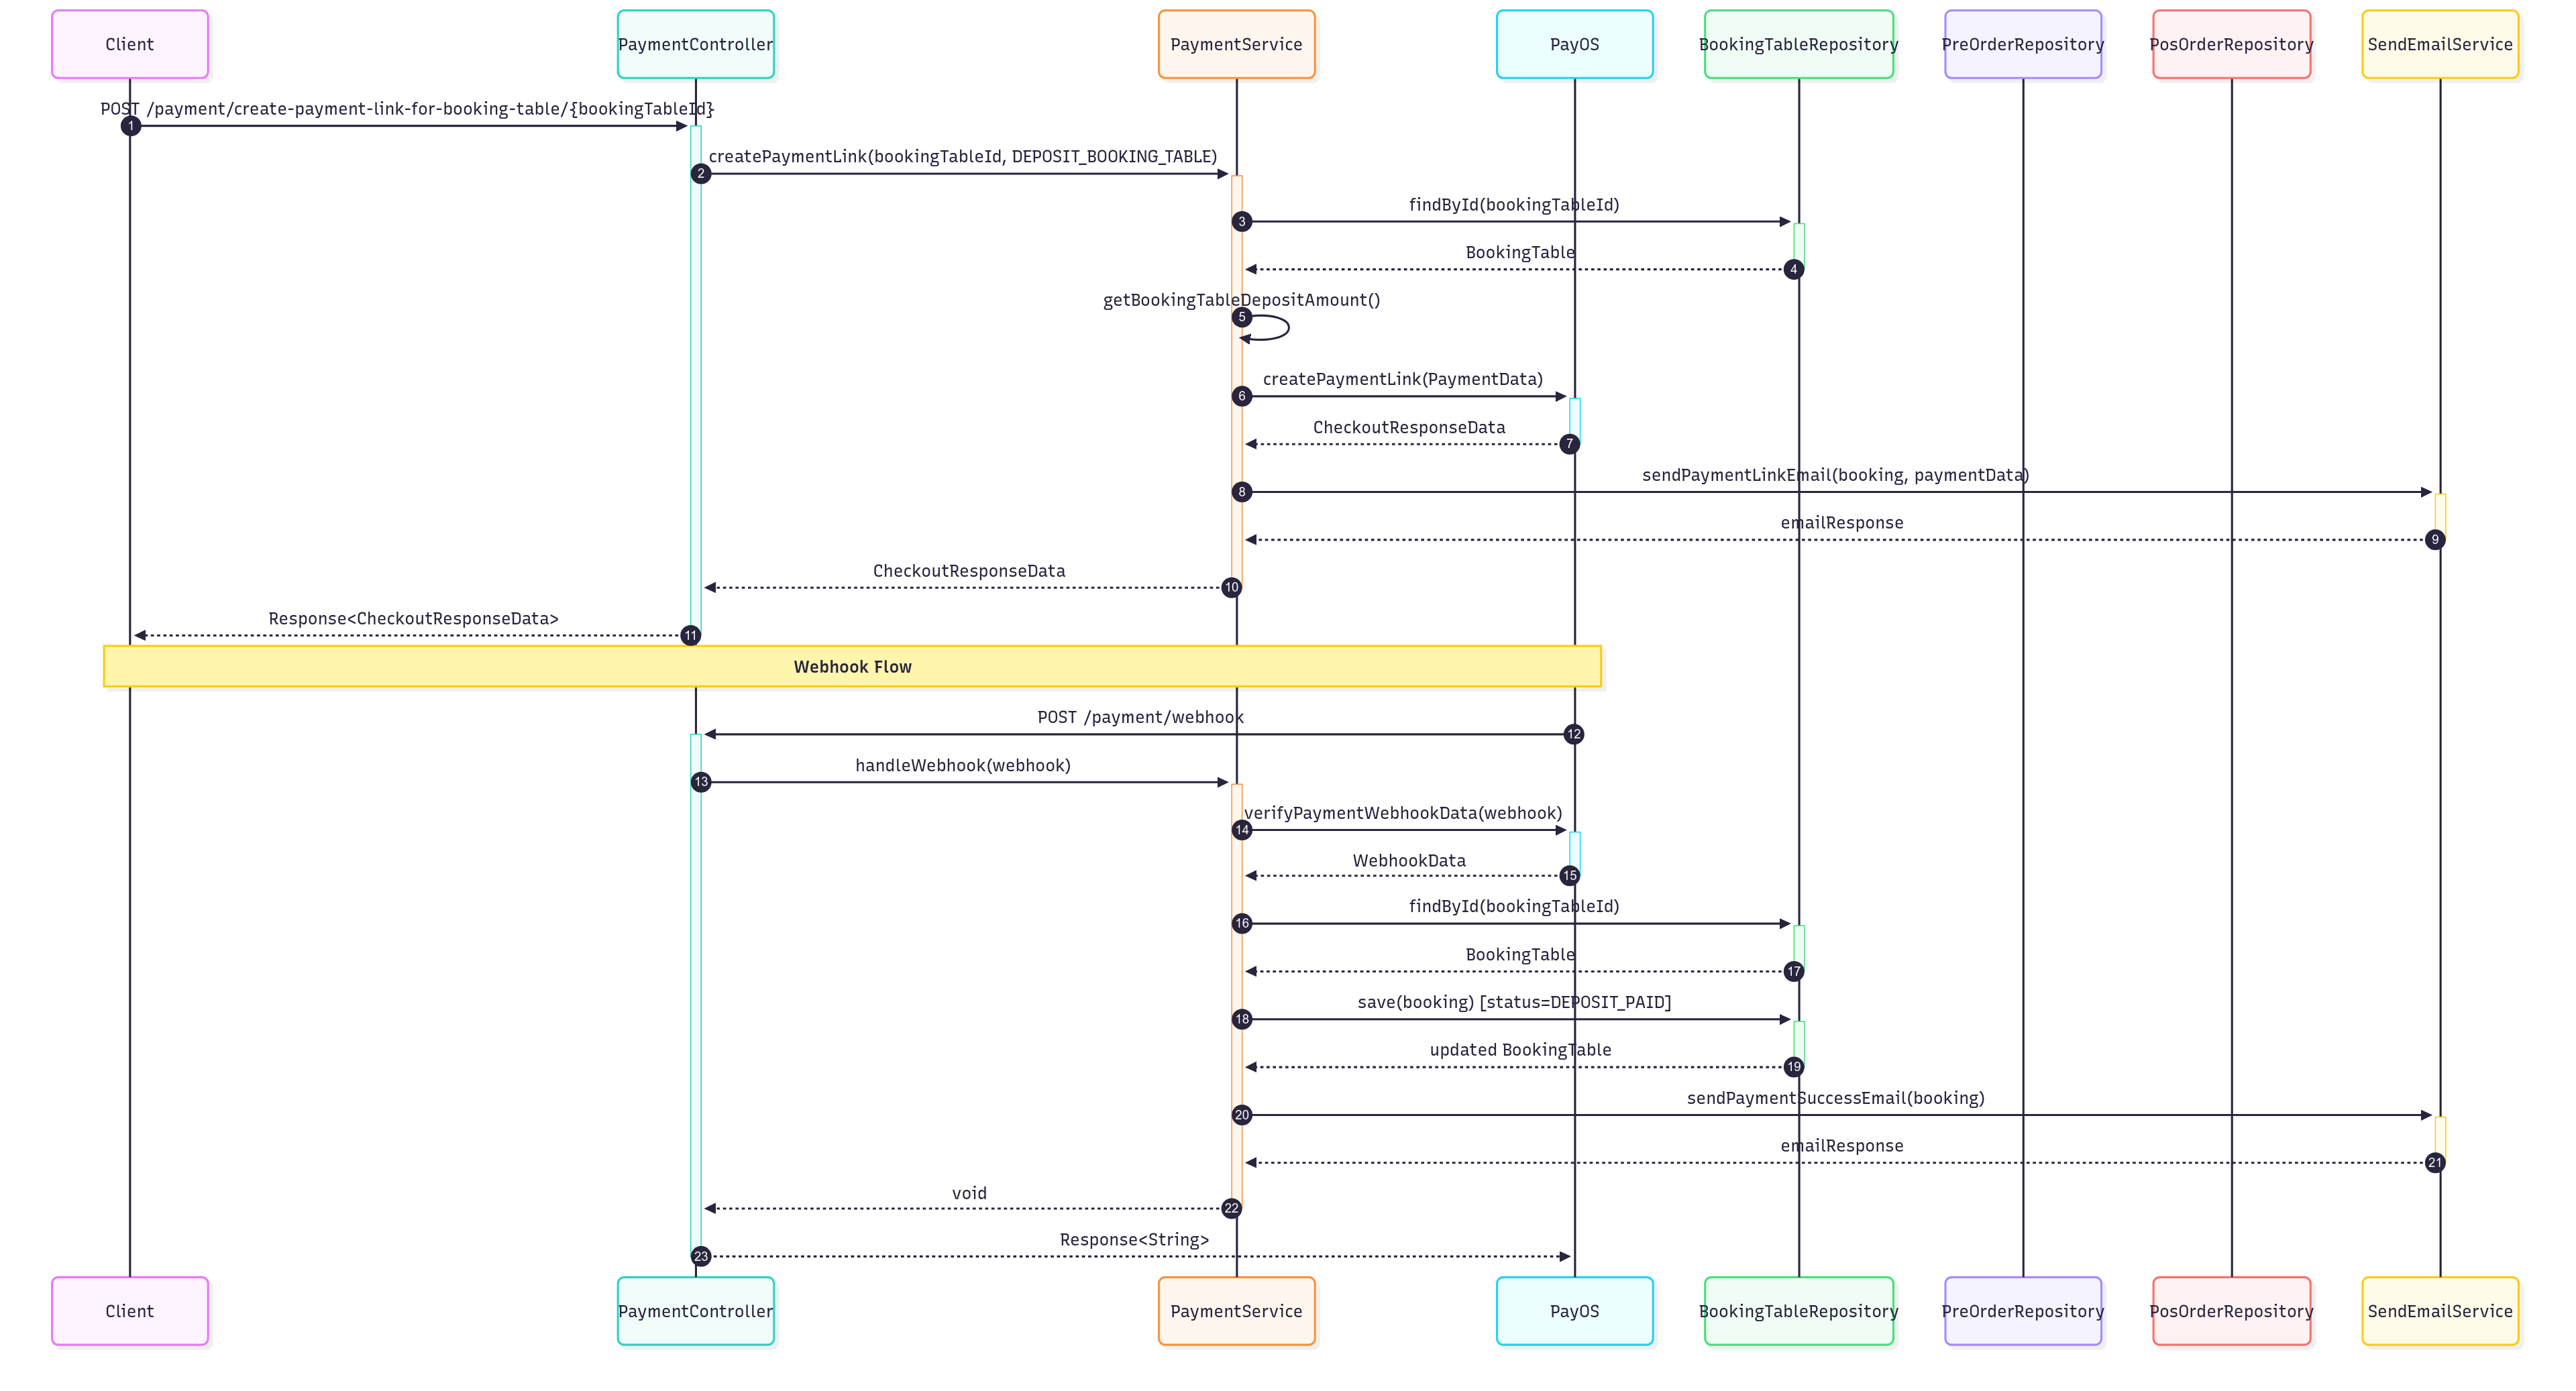
\includegraphics[width=\linewidth]{Images/diagram/Payment_sequence}
    \vspace{0.5cm}
    \caption{Sequence diagram: Thanh toán}
    \label{fig:my_label}
\end{figure}
\begin{figure}[H]
    \centering
    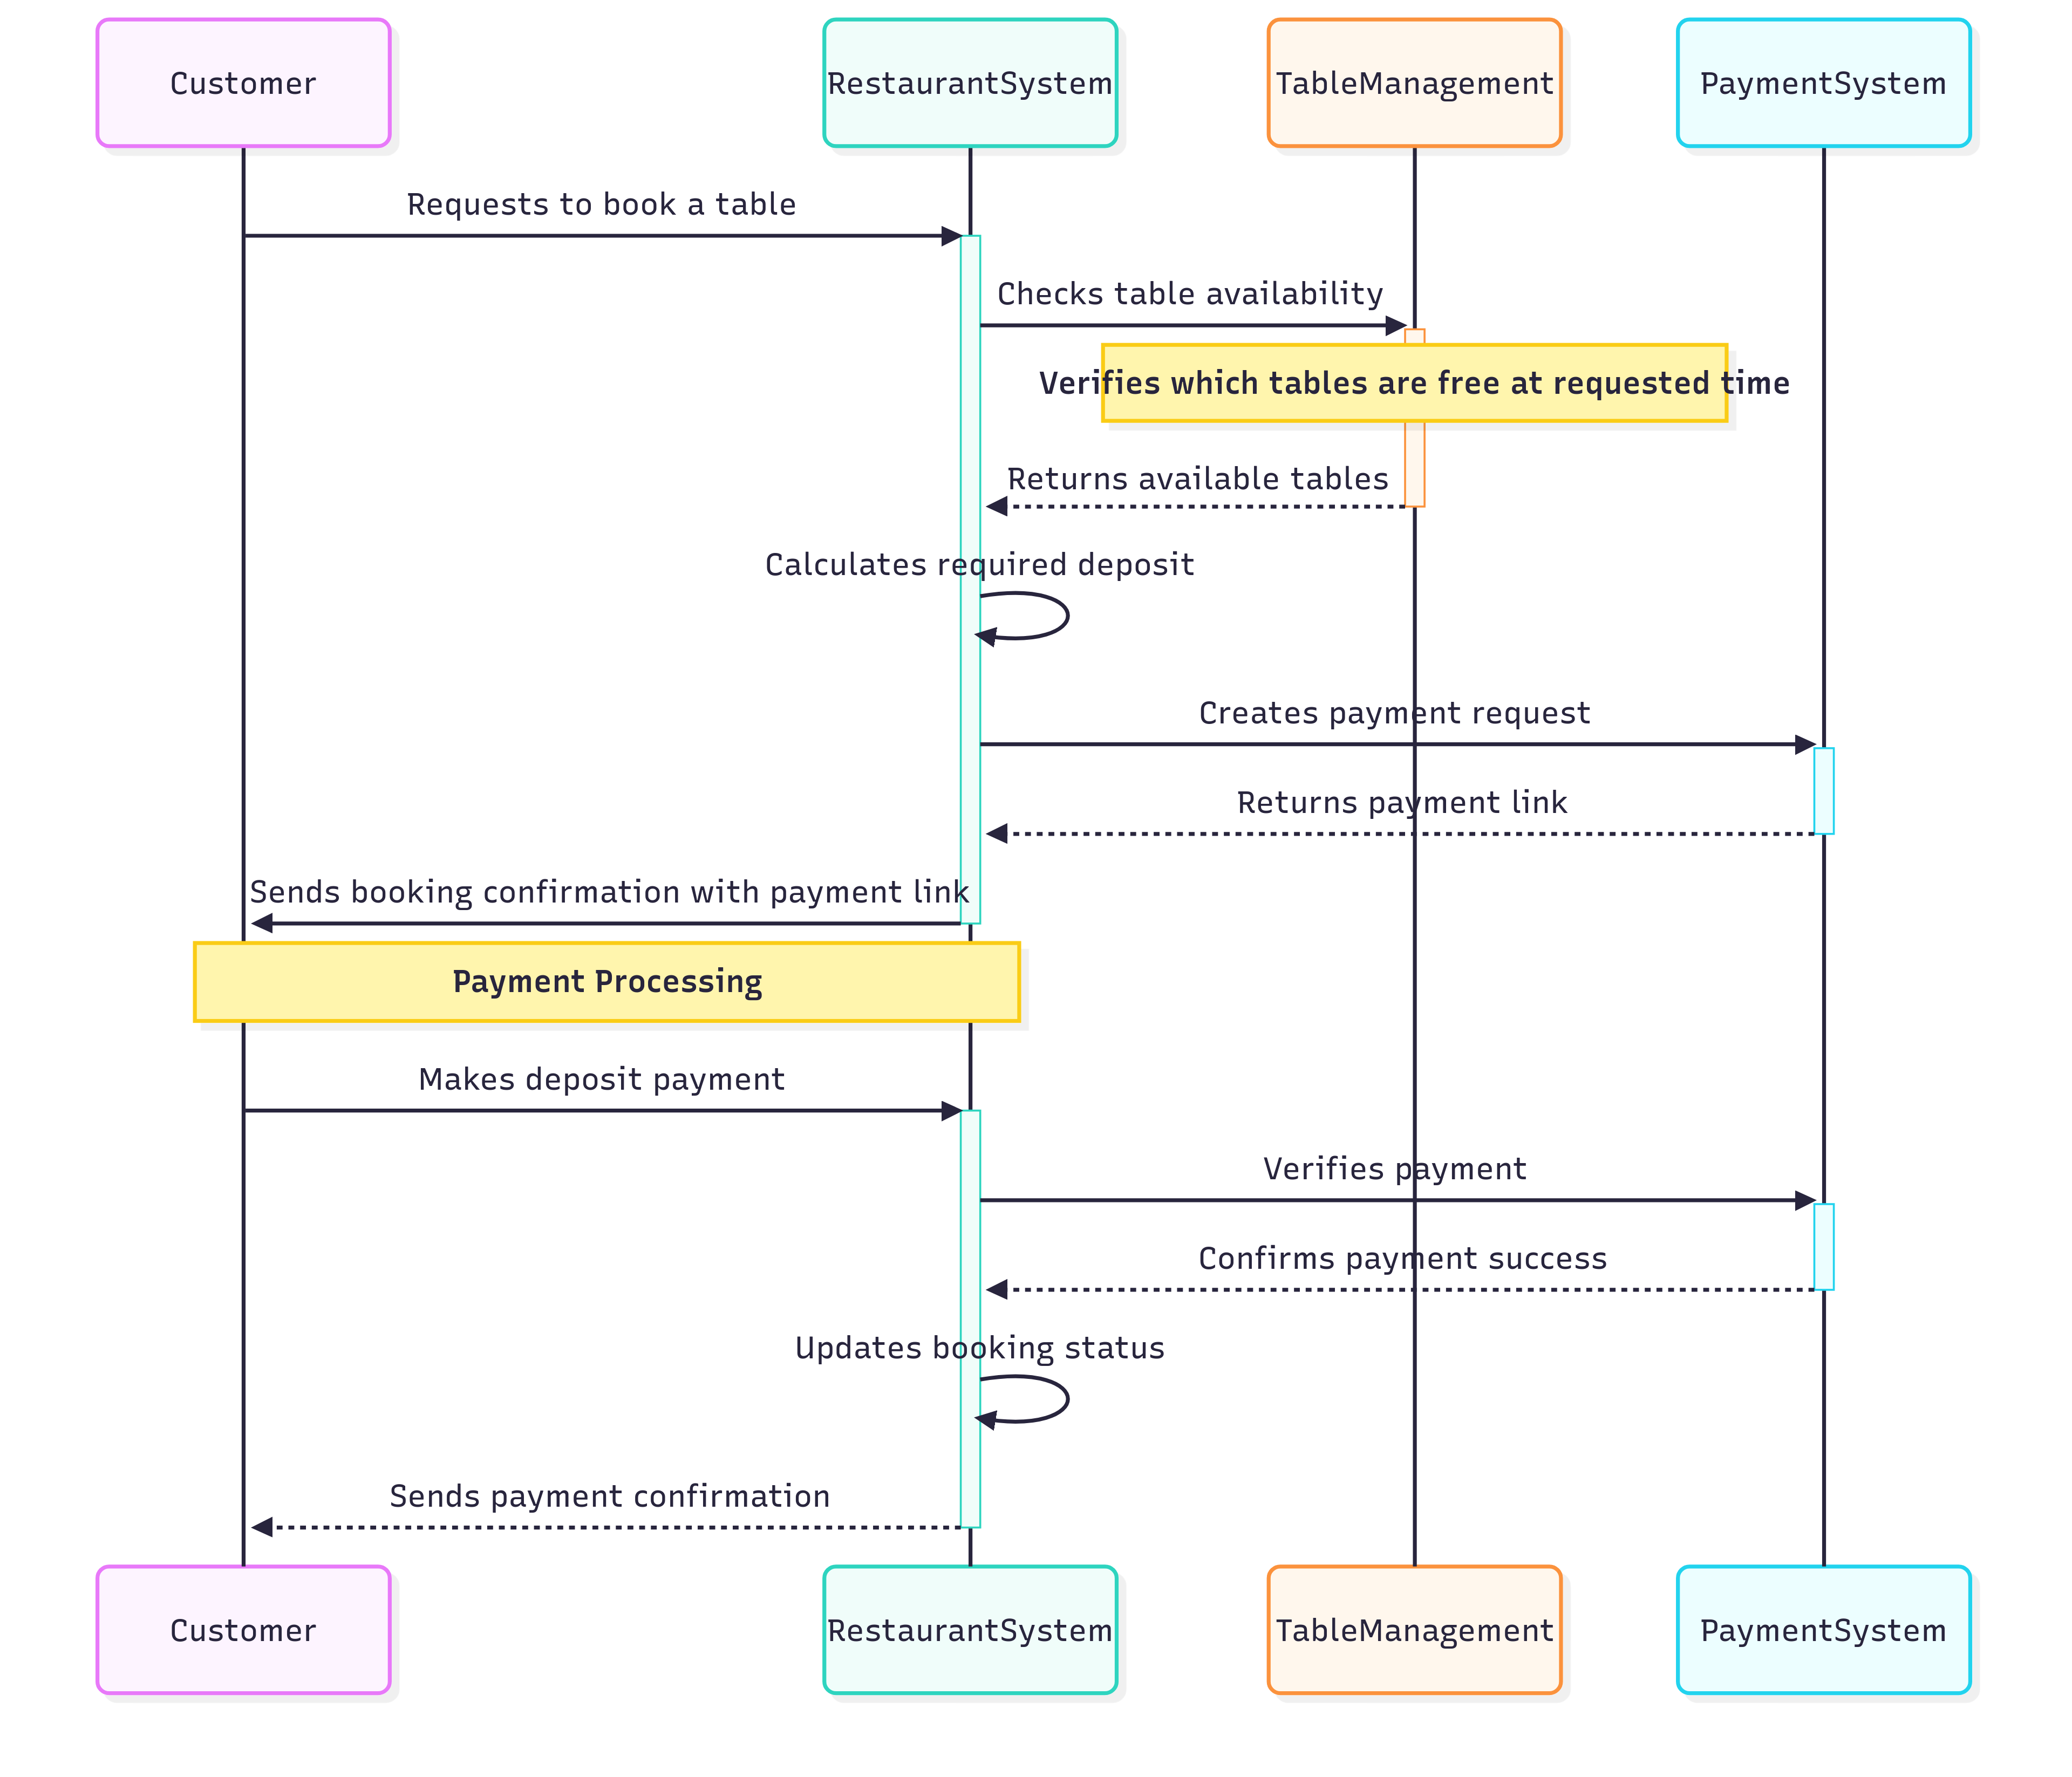
\includegraphics[width=\linewidth]{Images/diagram/Booking_sequence}
    \vspace{0.5cm}
    \caption{Sequence diagram: Đặt bàn}
    \label{fig:my_label}
\end{figure}


\subsection{Giao diện người dùng}
\begin{itemize}
	\item \textbf{Trang chủ (Homepage)}  
	\begin{figure}[H]
        \centering
        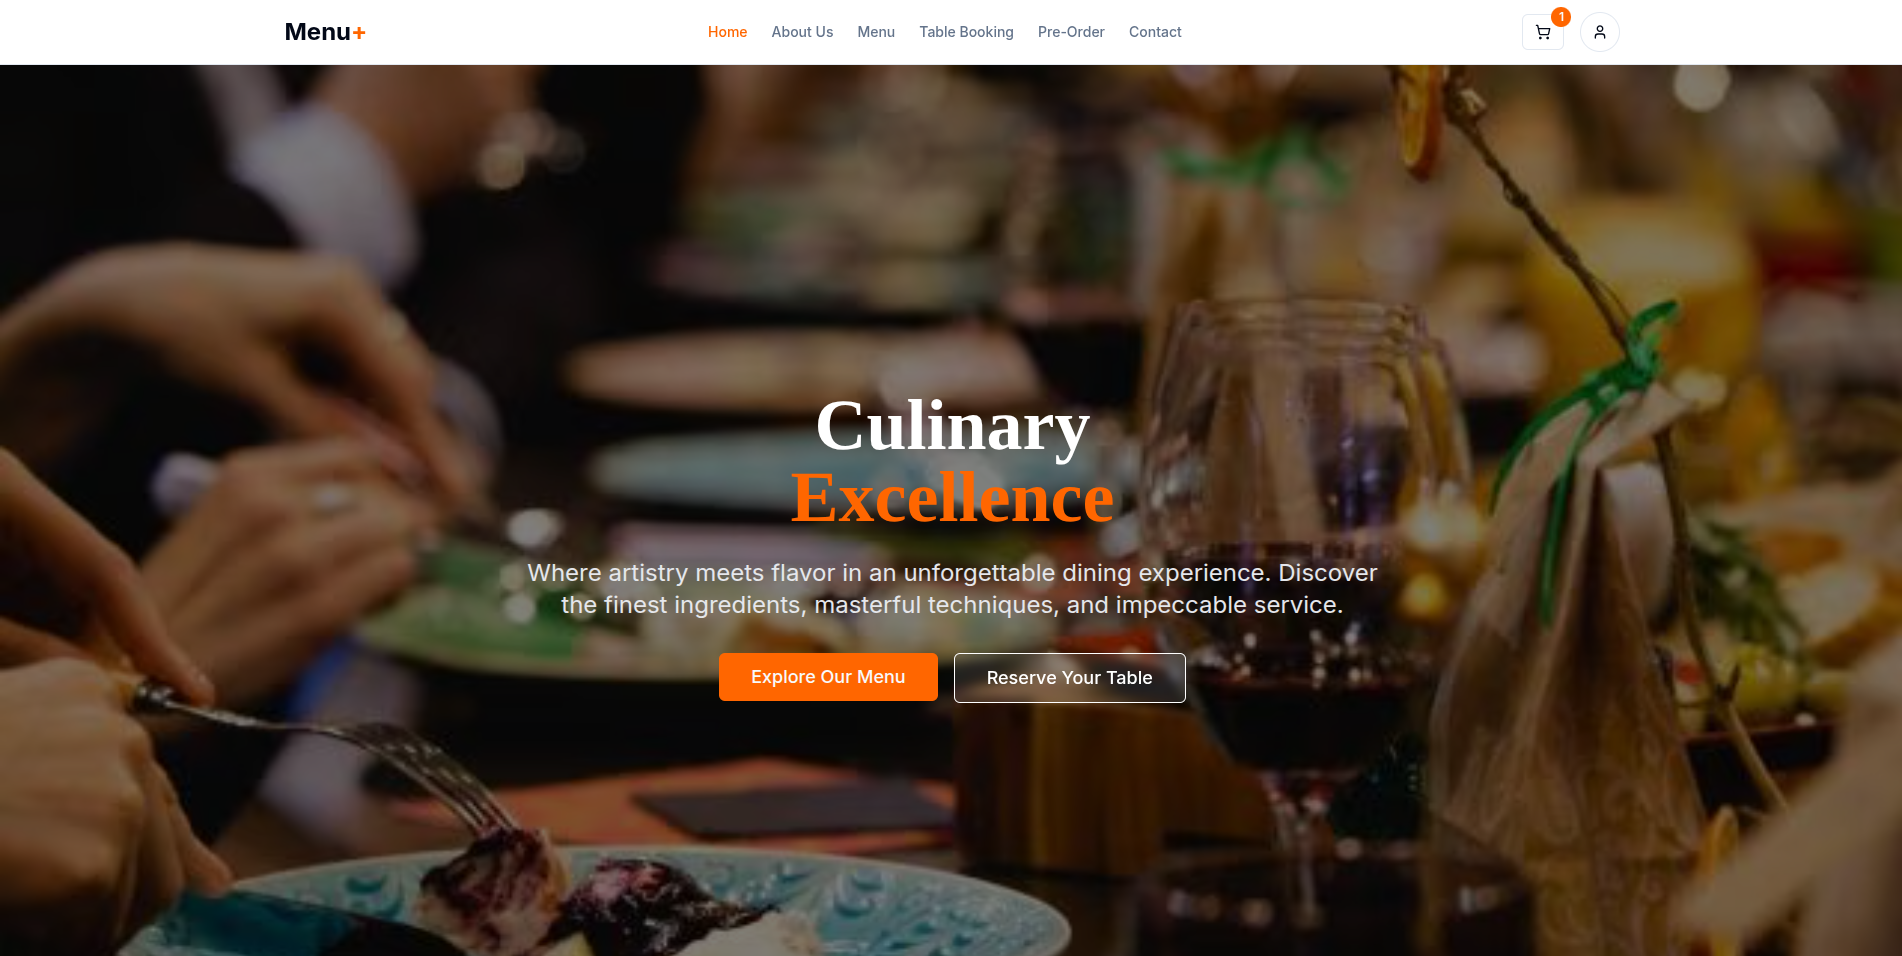
\includegraphics[width=15cm]{Images/hienthuc/homepage.png}
        \vspace{0.5cm}
        \caption{Trang chủ}
        \label{fig:homepage}
    \end{figure}
	Trang chủ giới thiệu nhà hàng, hiển thị các nút điều hướng chính như Menu, Đặt bàn, Pre-Order, và Contact. Người dùng có thể nhanh chóng khám phá thực đơn hoặc đặt bàn.

	\item \textbf{Đặt bàn (Table Booking)}  
	\begin{figure}[H]
        \centering
        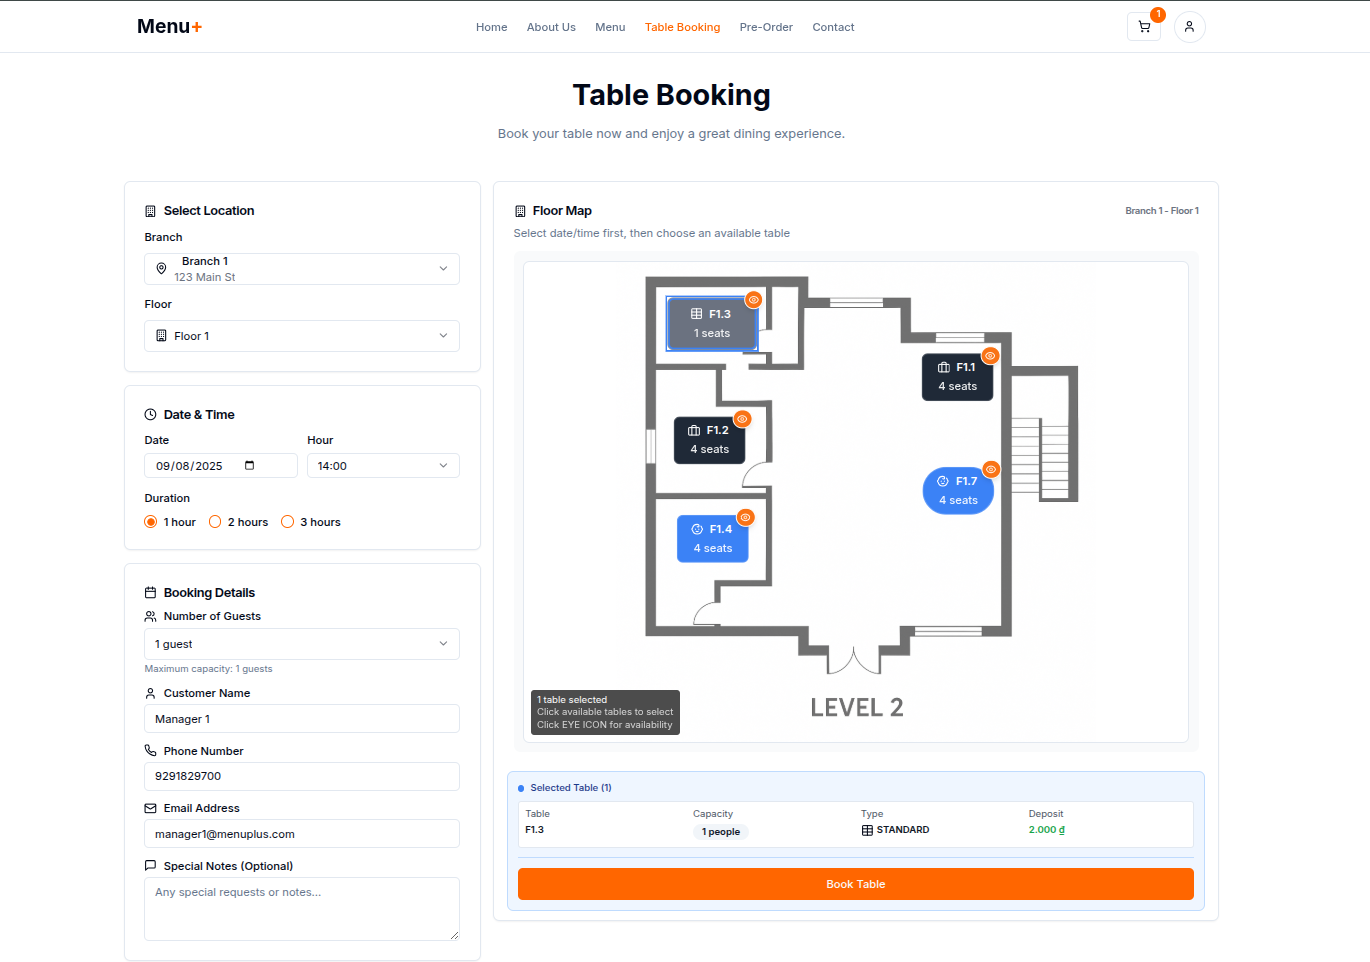
\includegraphics[width=15cm]{Images/hienthuc/bookingtable.png}
        \vspace{0.5cm}
        \caption{Đặt bàn}
        \label{fig:bookingtable}
    \end{figure}
	Khách hàng chọn chi nhánh, tầng, thời gian, số lượng khách. Sơ đồ bàn trực quan cho phép chọn bàn còn trống, kèm thông tin chi tiết về bàn và khoản đặt cọc.

	\item \textbf{Quản lý sơ đồ bàn (Floor Setup)}  
	\begin{figure}[H]
        \centering
        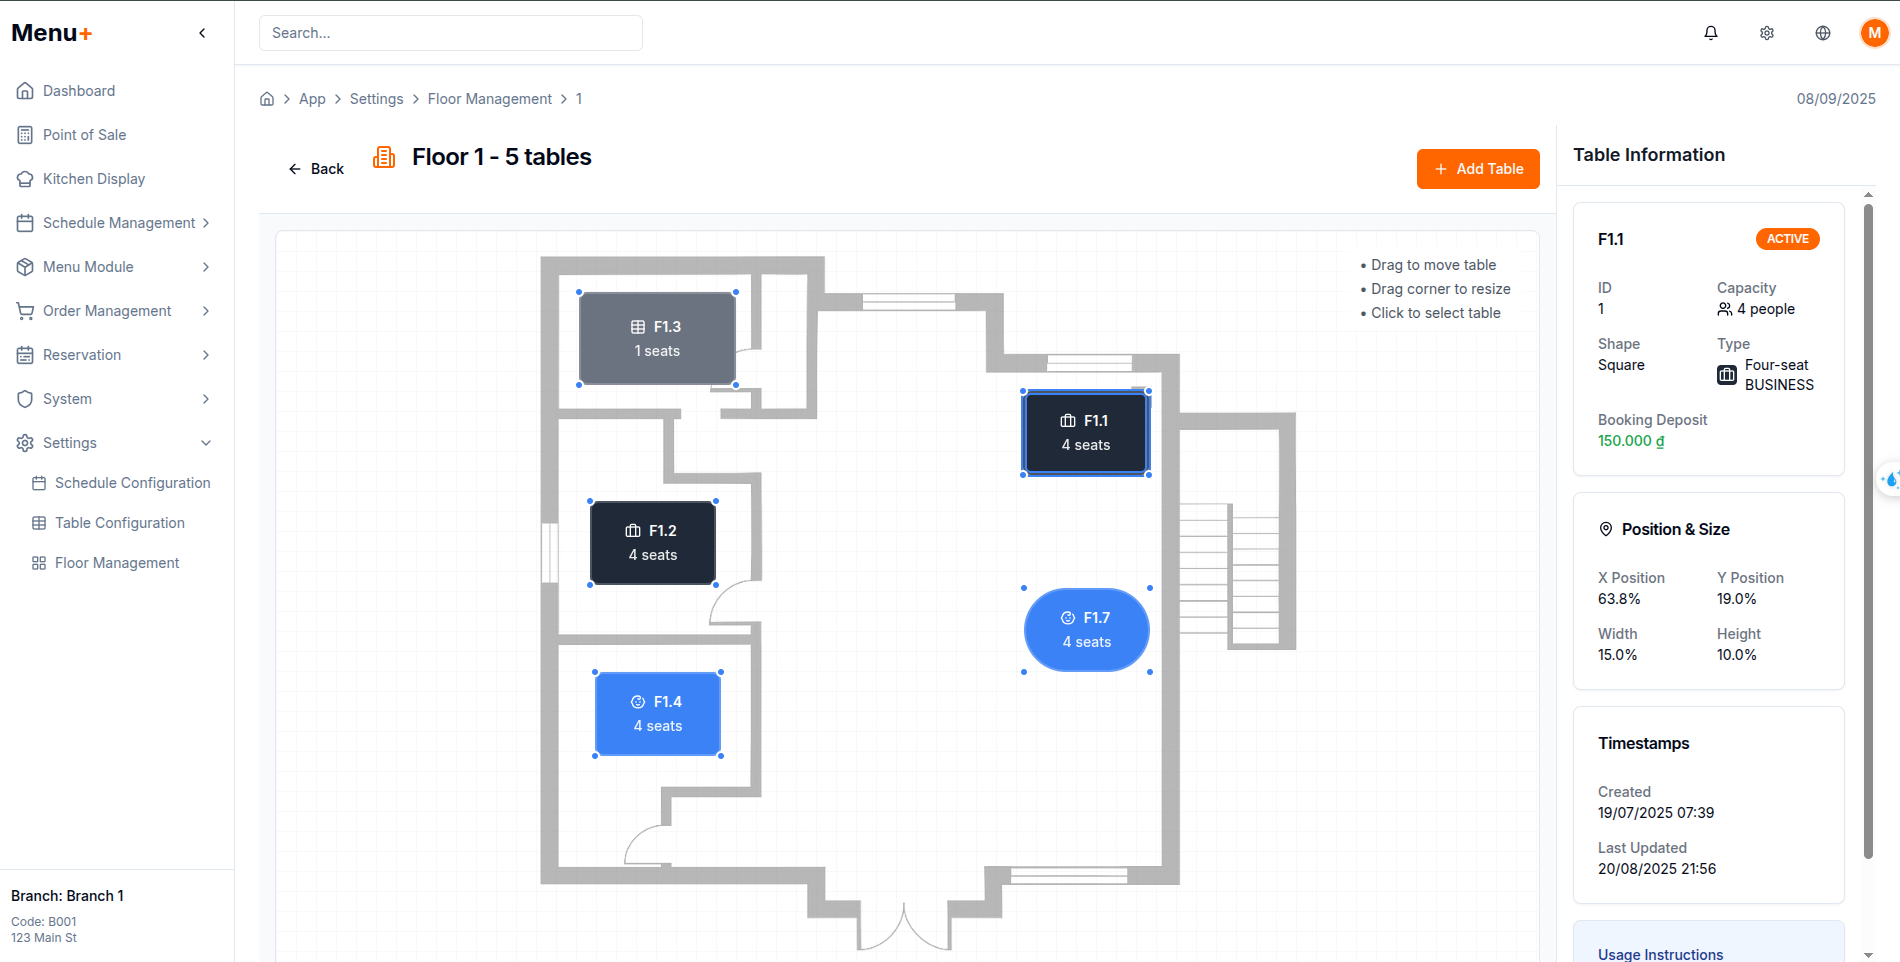
\includegraphics[width=15cm]{Images/hienthuc/floorsetup.png}
        \vspace{0.5cm}
        \caption{Quản lý sơ đồ bàn}
        \label{fig:floorsetup}
    \end{figure}
	Quản trị viên có thể thêm/sửa/xóa bàn, thay đổi vị trí và kích thước trên sơ đồ mặt bằng. Mỗi bàn có thông tin chi tiết: sức chứa, loại bàn, trạng thái hoạt động, tiền đặt cọc.

	\item \textbf{Xem chi tiết món ăn (Food Detail)}  
	\begin{figure}[H]
        \centering
        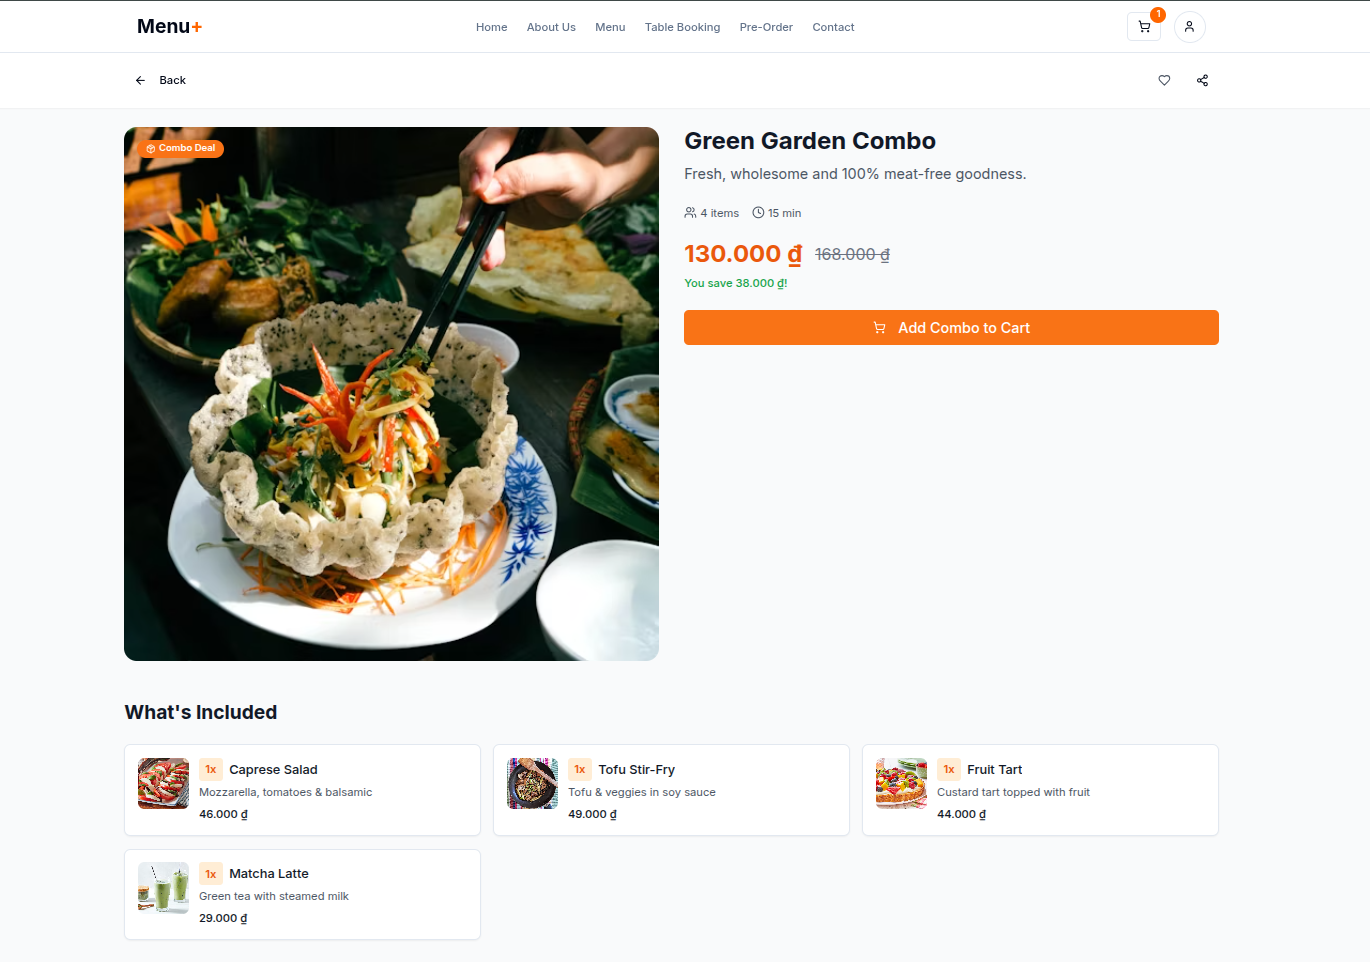
\includegraphics[width=15cm]{Images/hienthuc/fooddetail.png}
        \vspace{0.5cm}
        \caption{Xem chi tiết món ăn}
        \label{fig:fooddetail}
    \end{figure}
	Người dùng xem thông tin chi tiết món ăn/combos, giá, thời gian chuẩn bị, và danh sách các món đi kèm. Cho phép thêm món vào giỏ hàng nhanh chóng.

	\item \textbf{Thực đơn (Menu)}  
	\begin{figure}[H]
        \centering
        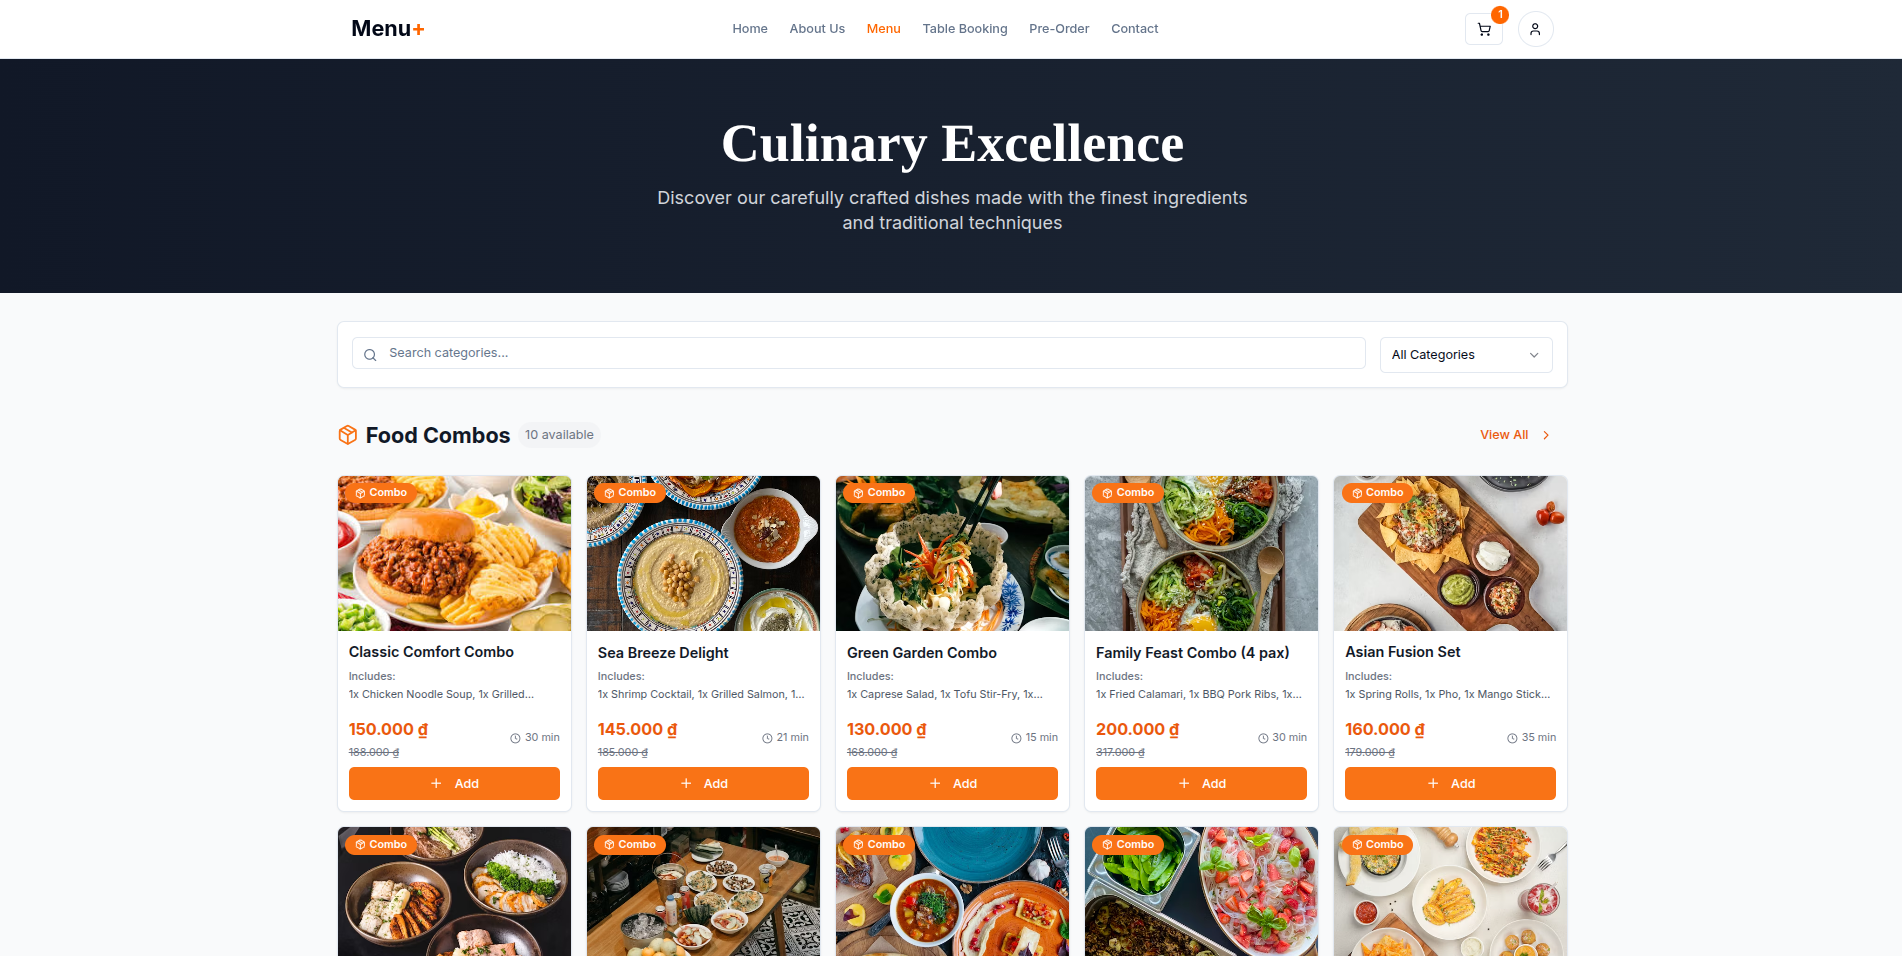
\includegraphics[width=15cm]{Images/hienthuc/menu.png}
        \vspace{0.5cm}
        \caption{Thực đơn}
        \label{fig:menu}
    \end{figure}
	Giao diện hiển thị danh sách món ăn, phân loại theo nhóm (đồ uống, món chính, combo, món tráng miệng,...). Người dùng dễ dàng tìm kiếm và thêm món vào giỏ.

	\item \textbf{Quản lý đơn hàng (Order Management)}  
	\begin{figure}[H]
        \centering
        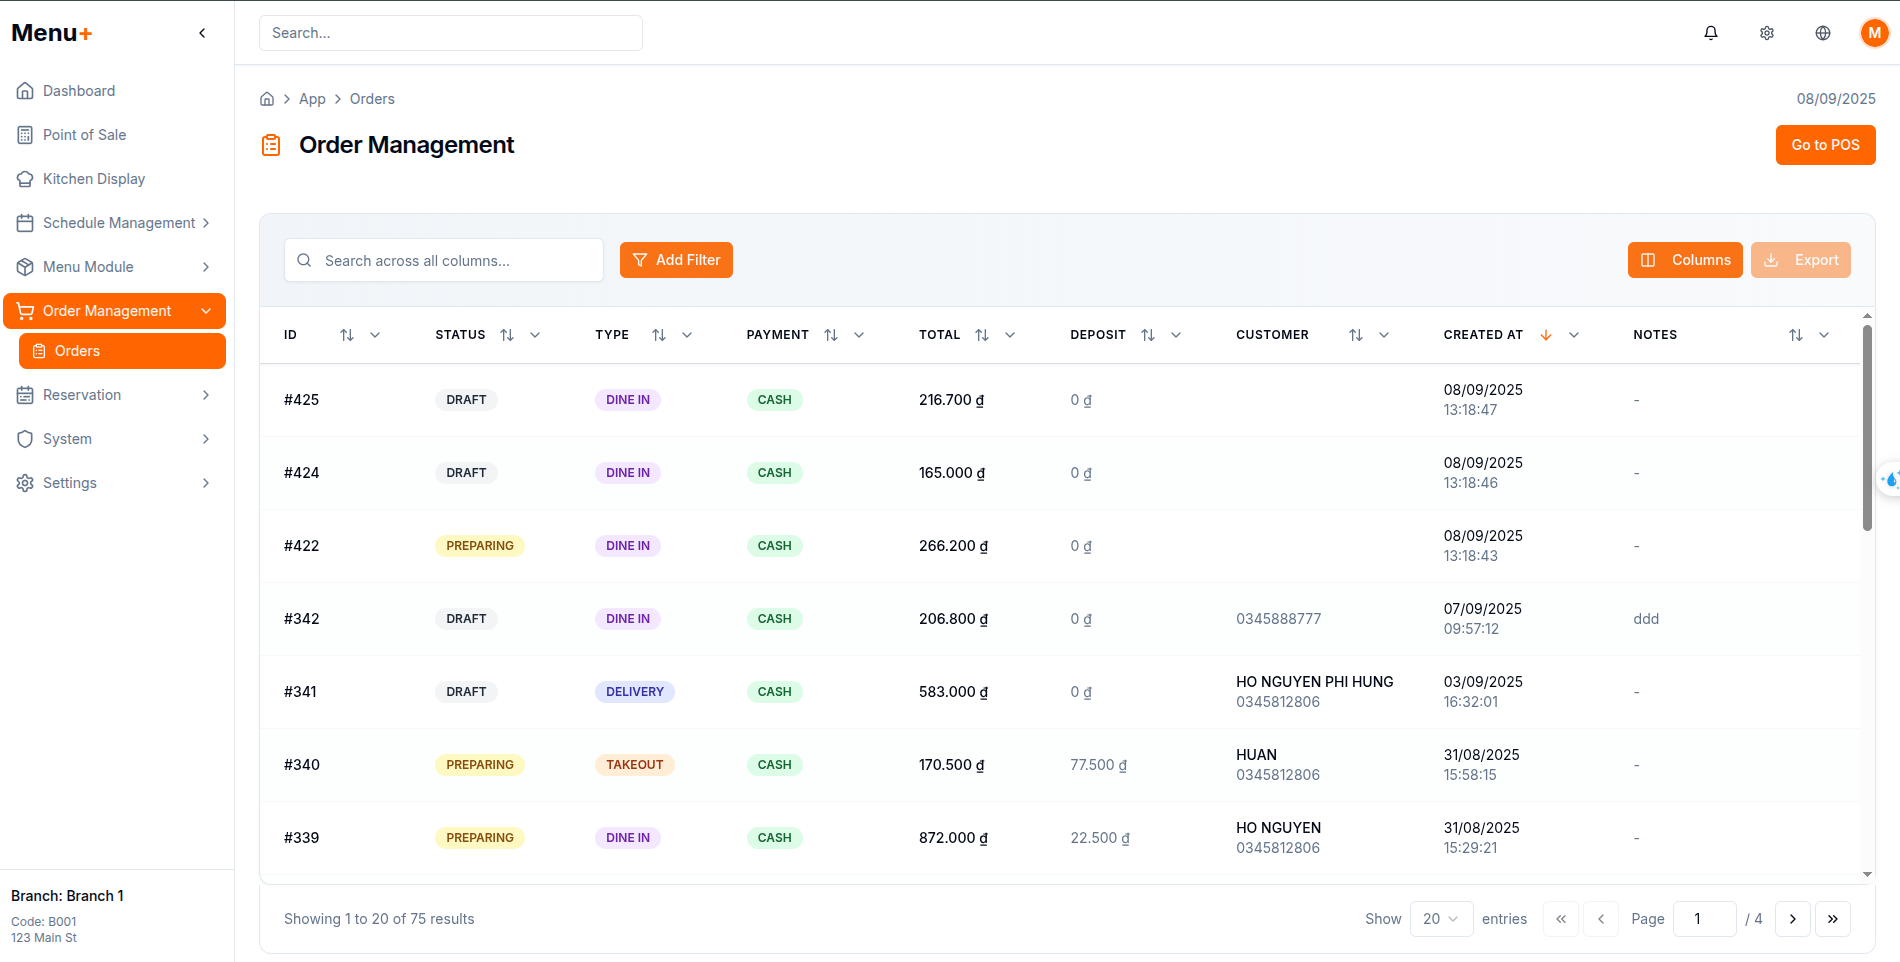
\includegraphics[width=15cm]{Images/hienthuc/ordermanage.png}
        \vspace{0.5cm}
        \caption{Quản lý đơn hàng}
        \label{fig:ordermanage}
    \end{figure}
	Quản trị viên theo dõi danh sách đơn hàng theo trạng thái (Draft, Preparing, Completed,...), kèm thông tin khách hàng, phương thức thanh toán, và tổng tiền.

	\item \textbf{Điểm bán hàng (POS - Point of Sale)}  
	\begin{figure}[H]
        \centering
        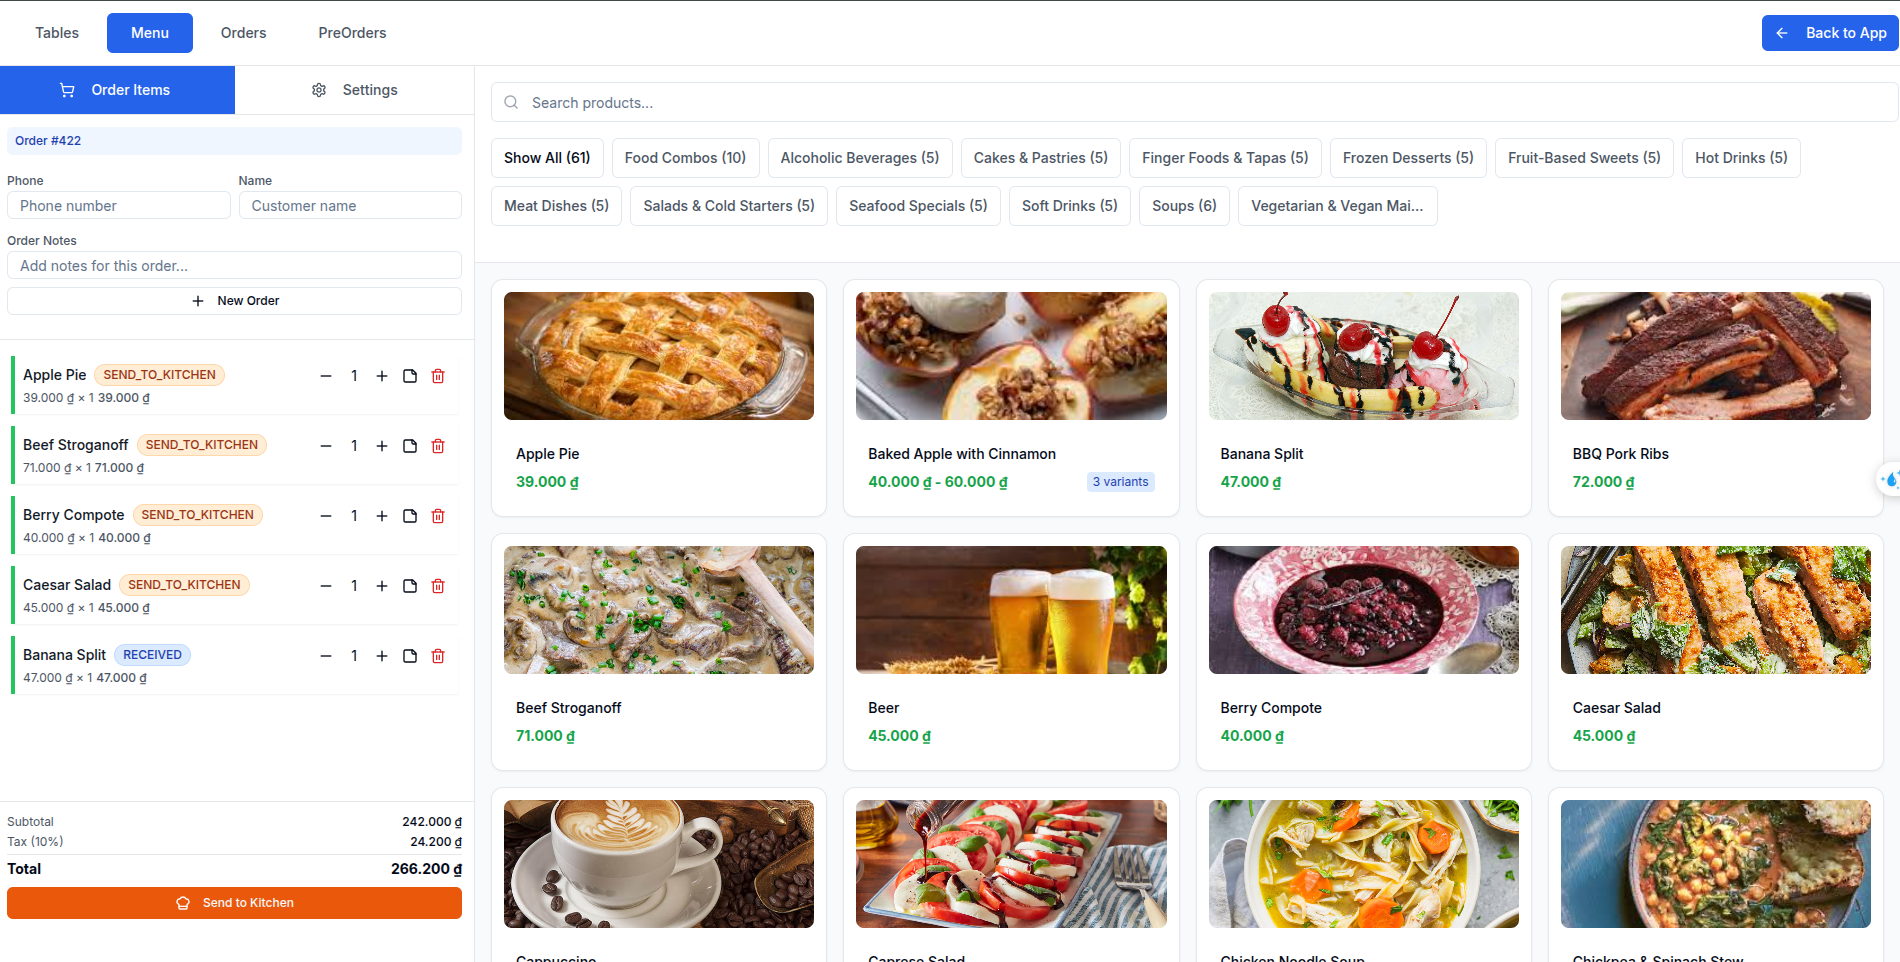
\includegraphics[width=15cm]{Images/hienthuc/pos.png}
        \vspace{0.5cm}
        \caption{Điểm bán hàng}
        \label{fig:pos}
    \end{figure}
	Giao diện dành cho nhân viên phục vụ: chọn món, thêm ghi chú, gửi order tới bếp. Đồng thời hiển thị giỏ hàng, tính tổng tiền và thuế.

	\item \textbf{Đặt món trước (Pre-Order)}  
	\begin{figure}[H]
        \centering
        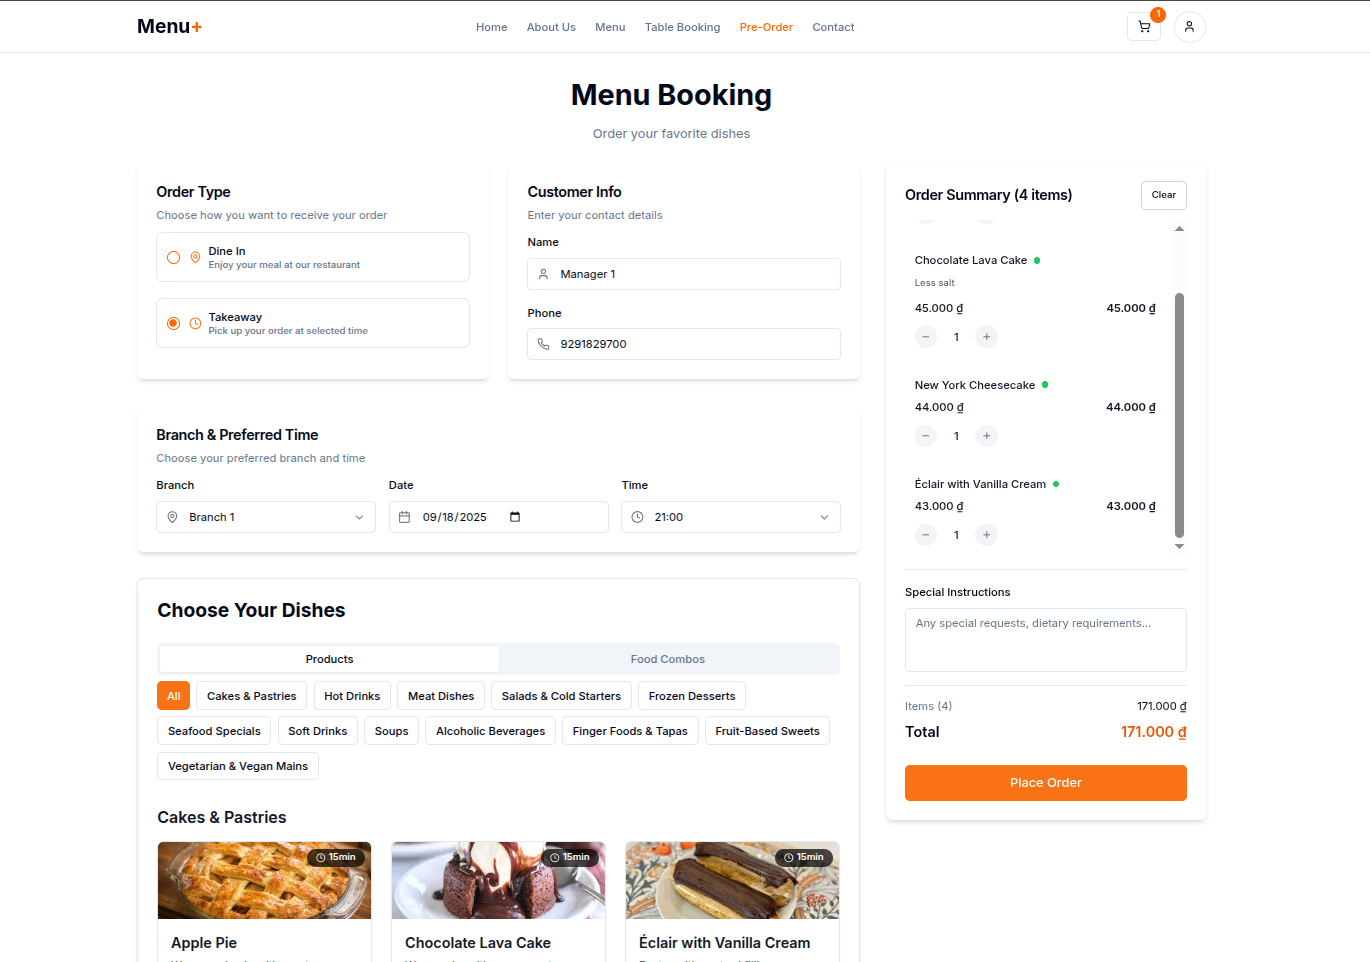
\includegraphics[width=15cm]{Images/hienthuc/preorder.png}
        \vspace{0.5cm}
        \caption{Đặt món trước}
        \label{fig:preorder}
    \end{figure}
	Khách hàng chọn loại hình (Dine In/Takeaway), chi nhánh, thời gian, và các món ăn. Phần tóm tắt đơn hàng hiển thị đầy đủ giá trị hóa đơn trước khi xác nhận.

	\item \textbf{Báo cáo bán hàng (Sales Report)}  
	\begin{figure}[H]
        \centering
        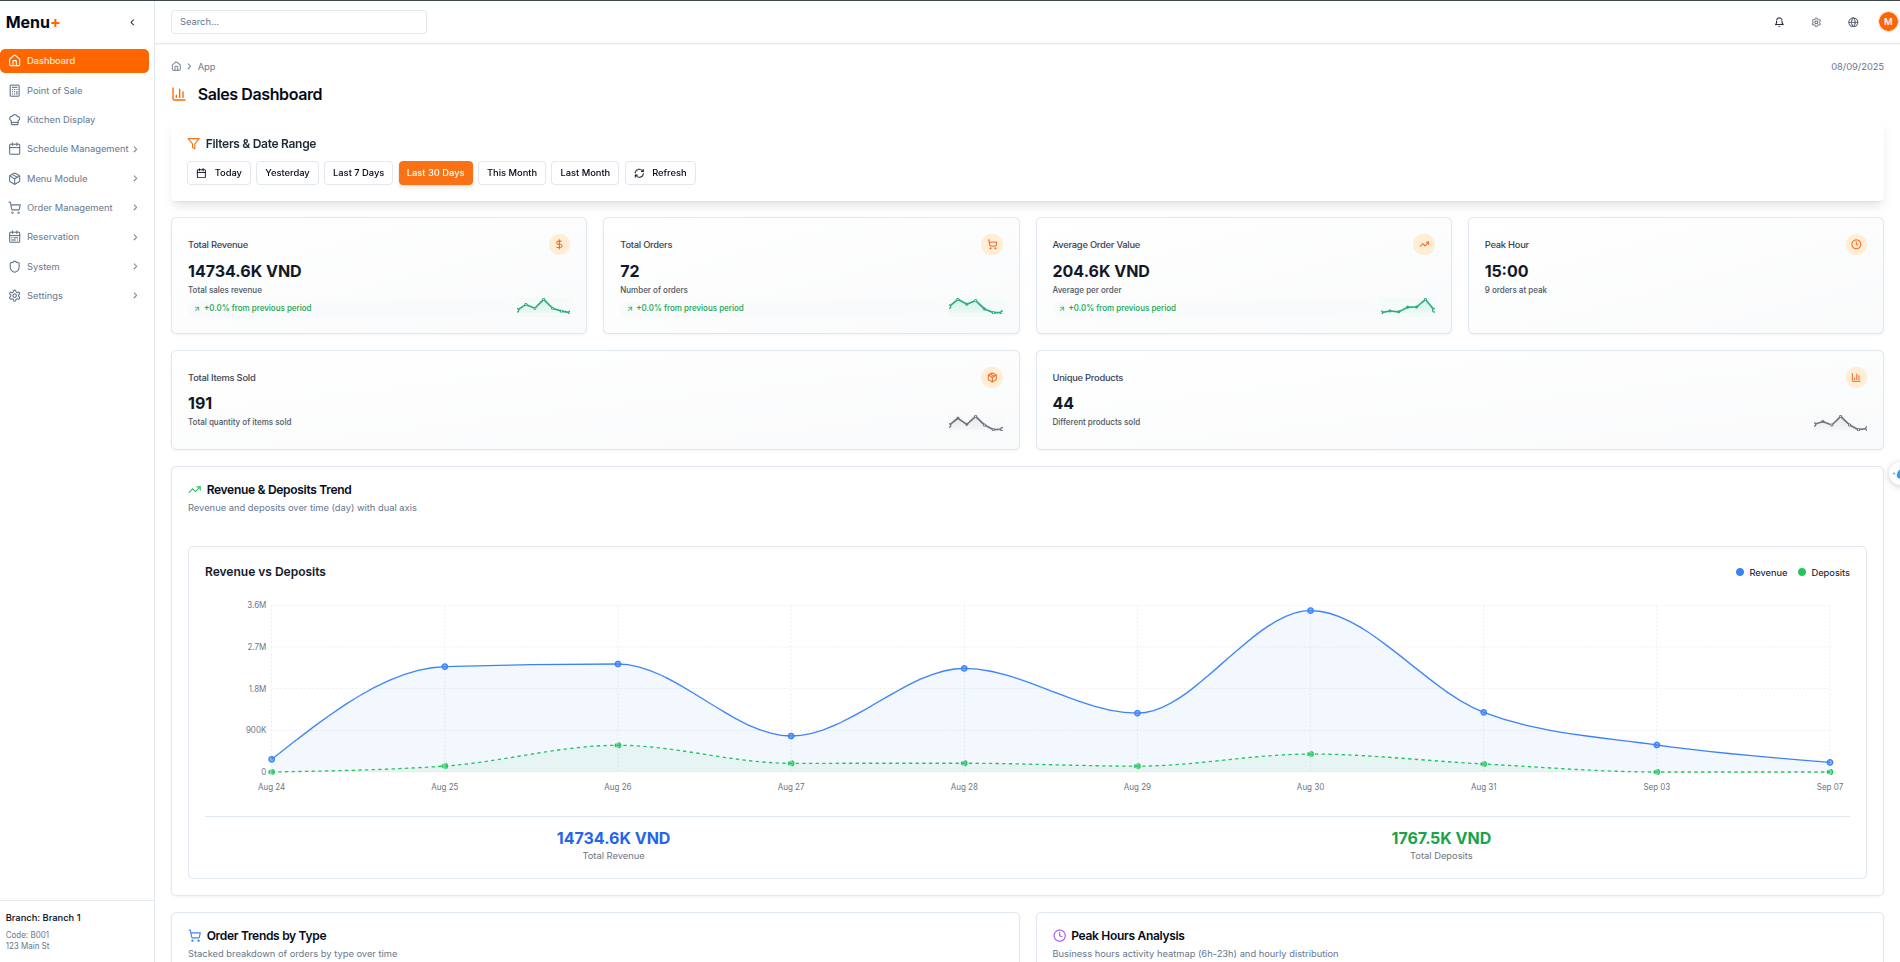
\includegraphics[width=15cm]{Images/hienthuc/salereport.png}
        \vspace{0.5cm}
        \caption{Báo cáo bán hàng}
        \label{fig:salereport}
    \end{figure}
	Giao diện dashboard thống kê doanh thu, số lượng đơn hàng, sản phẩm bán chạy, xu hướng theo ngày/tuần/tháng, giúp quản lý dễ dàng phân tích hiệu quả kinh doanh.

	\item \textbf{Quản lý lịch làm việc (Schedule Manager)}  
	\begin{figure}[H]
        \centering
        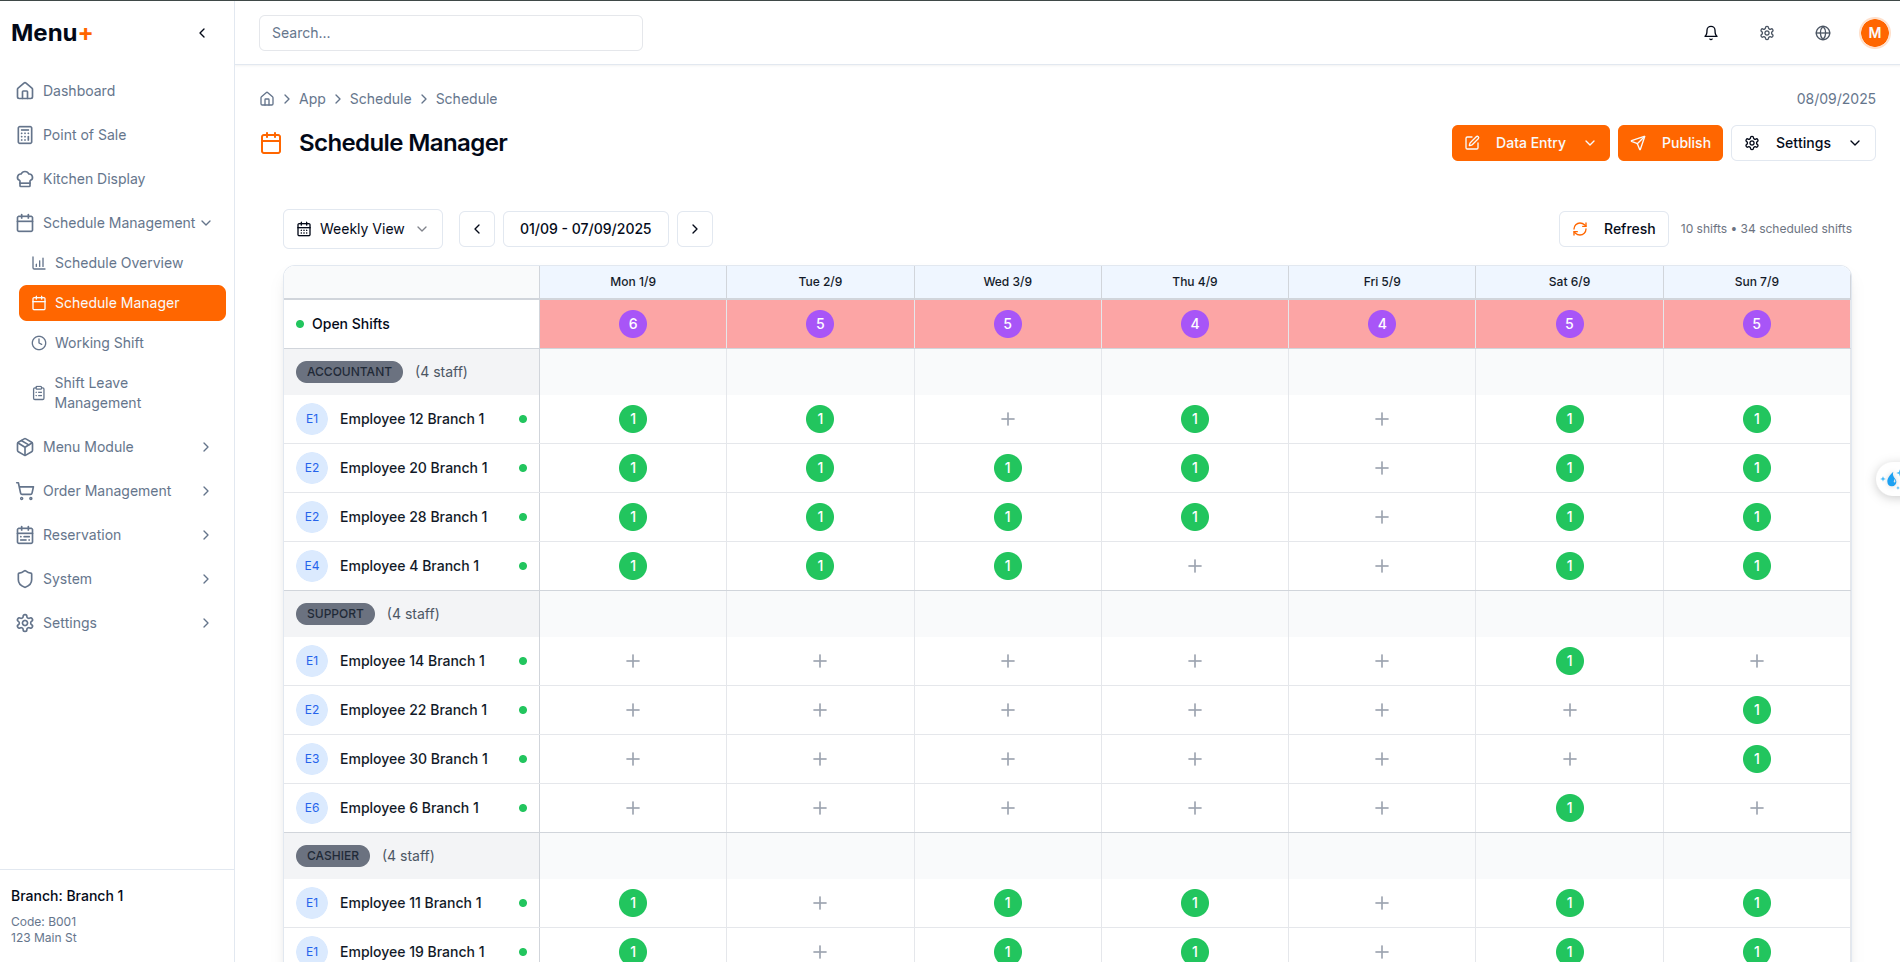
\includegraphics[width=15cm]{Images/hienthuc/schedule.png}
        \vspace{0.5cm}
        \caption{Quản lý lịch làm việc}
        \label{fig:schedule}
    \end{figure}
	Quản lý ca làm việc của nhân viên theo tuần. Người quản trị có thể phân công ca, xem lịch trống, và quản lý ca nghỉ phép.
\end{itemize}
